\documentclass[output=paper]{langscibook} 
\title{Repairing Final-Over-Final Constraint Violations: \\Evidence from Basque verb clusters} 
\author{%
 Ricardo Etxepare\affiliation{IKER UMR 5478-CNRS}  
 \lastand 
 Bill Haddican\affiliation{CUNY, Queens College/Graduate Center}
}

\abstract{
This article discusses implications of Basque modal constructions for representational models of Final-Over-Final Constraint (FOFC) effects.  We argue that FOFC-violating structures at an intermediate derivational level can be repaired by subsequent movement steps.  The analysis entails that FOFC-violating structures are buildable by the syntax, contra narrow syntactic approaches to FOFC, and that FOFC evaluation instead applies in the phonology after copy deletion.  Such a view of FOFC helps explain several recalcitrant word order restrictions on Basque modal constructions as well as variation in the effect of focus and negation on modal placement across Basque dialects.
}

% linguistic trees: 
\usepackage{qtree} %http://tug.ctan.org/tex-archive/macros/latex/contrib/qtree/

% IPA symbols:
%\usepackage{tipa} %http://tug.ctan.org/tex-archive/fonts/tipa/

% linguistic examples:
%\usepackage{linguex} %http://tug.ctan.org/tex-archive/macros/latex/contrib/linguex/

% suppresses the dash in references to subexamples (linguex.sty)
%\renewcommand{\refdash}{}

%additional packages
\usepackage{etex}
\usepackage{float}
\usepackage{tikz}
\usepackage{tikz-qtree}
%\usepackage{amssymb}
\usepackage[icelandic, swedish, american]{babel}
%\usepackage[T1]{fontenc}
%\usepackage[utf8]{inputenc}
\usepackage{linguex}
%\usepackage{langsci-gb4e}
%\renewcommand{\refdash}{}
\usepackage{tabularx}
%\usepackage{color}
%\usepackage{ulem}
\usepackage{soul}
%\usepackage{biblatex}
\usepackage{multicol}
%\usepackage[demo]{graphicx}
\usepackage[justification=raggedright,singlelinecheck=false]{caption}
\usepackage[justification=raggedright,singlelinecheck=false]{subcaption}
\renewcommand{\firstrefdash}{}
%\usepackage{natbib}

%\usepackage{langsci-gb4e}
%\usepackage{langsci-cgloss}


%
\bibliography{anders}

\begin{document}

\maketitle

%%% ENTER A BRIEF TITLE: this appears in the running head
%\brieftitle{Reparing Final-Over-Final Constraint Violations}

%\runninghead


%%% ENTER AN ACKNOWLEDGMENT, which will be the first, unnumbered footnote:
%\ackfootnote{We would like to thank ...}


%%% REPLACE ABSTRACT TEXT WITH YOUR OWN ABSTRACT
%\noindent \textit{Abstract}. %{This paper discusses implications of Basque modal constructions for representational models of Final-Over-Final Constraint (FOFC) effects.  We argue that FOFC-violating structures at an intermediate derivational level can be repaired by subsequent movement steps.  The analysis entails that FOFC-violating structures are buildable by the syntax, contra narrow syntactic approaches to FOFC, and that FOFC evaluation instead applies in the phonology after copy deletion.  Such a view of FOFC helps explain several recalcitrant word order restrictions on Basque modal constructions as well as variation in the effect of focus and negation on modal placement across Basque dialects.}


\section{Introduction} \protect\label{introduction}
This article discusses some implications of Basque modal constructions for recent approaches to  Final-Over-Final Constraint (FOFC) effects.  FOFC is a  generalization originally by \cite{holmberg2000} about the interaction between dominance relations and \{head, complement\} ordering cross-linguistically.   In particular, following much previous typological literature, Holmberg  noted that  ``harmonic'' sequences of  head-final, and head-initial phrases, as in \Next[a,b] are common cross-linguistically, as are ``disharmonic'' sequences where a head-initial phrase dominates a head-final phrase, as in \Next[c] \citep{hawkins1983, hawkins1995}.  Holmberg noted that what is much rarer---possibly unattested in relevant domains---are instances of a head-final phrase dominating a head-initial phrase, as in \Next[d].


{\ex.\protect\label{fofcstructures}

\vspace*{-1cm}\begin{figure}[h!]
%\centering
\begin{subfigure}{.25\textwidth}
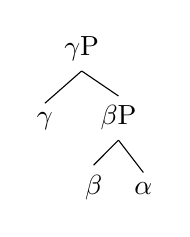
\begin{tikzpicture}[baseline]\tikzset{level distance=25pt, sibling distance=5pt}
\Tree
[.$\gamma$P $\gamma$ [.$\beta$P $\beta$ $\alpha$ ] ]
\end{tikzpicture}
  \caption{Harmonic, right-branching}
  \label{fig:sub1}
\end{subfigure}\hfill
\begin{subfigure}{.25\textwidth}
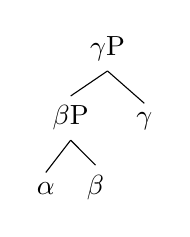
\begin{tikzpicture}[baseline]\tikzset{level distance=25pt, sibling distance=5pt}
\Tree
[.$\gamma$P [.$\beta$P $\alpha$ $\beta$ ] $\gamma$ ]
\end{tikzpicture}
  \caption{Harmonic, left-branching}
  \label{fig:sub2}
\end{subfigure}\hfill
\begin{subfigure}{.25\textwidth}
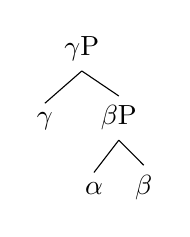
\begin{tikzpicture}[baseline]\tikzset{level distance=25pt, sibling distance=5pt}
\Tree
[.$\gamma$P $\gamma$ [.$\beta$P $\alpha$ $\beta$ ] ]
\end{tikzpicture}
  \caption{Disharmonic, attested}
  \label{fig:sub1}
\end{subfigure}\hfill
\begin{subfigure}{.22\textwidth}
 % \centering
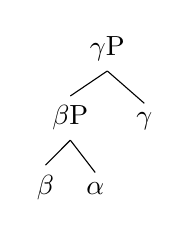
\begin{tikzpicture}[baseline]\tikzset{level distance=25pt, sibling distance=5pt}
\Tree
[.$\gamma$P [.$\beta$P $\beta$ $\alpha$ ] $\gamma$ ]
\end{tikzpicture}
%  \includegraphics[width=.4\linewidth]{image1}
  \caption{Disharmonic, unattested (in relevant domains)}
  \label{fig:sub2}
\end{subfigure}%
\end{figure}

}




For the moment, let us summarize Holmberg's observation about the above interaction as in \Next (taken from \cite{biberaueretal2014}).

\ex. \textbf{\textit{The Final-over-Final constraint}} (preliminary version)\\ \protect\label{fofc1}
If $\beta$ is a head-initial phrase and  $\gamma$ is a phrase immediately dominating $\beta$, then $\gamma$ must
be head-initial. If $\beta$ is a head-final phrase, and  $\gamma$ is a phrase immediately dominating
$\beta$, then  $\gamma$ can be head-initial or head-final.\\
(adapted from \cite{biberaueretal2014})


Following \cite{holmberg2000}, a now-considerable body of literature has described FOFC-effects cross-linguistically 
 \citep{holmberg2000,biberaueretal2008,biberaueretal2014, sheehan2013, sheehan2012} and diachronically \citep{biberaueretal2009, biberaueretal2010}. Formal approaches to FOFC effects have generally been of two types.\footnotemark\protect\footnotetext{We do not consider consider here' Hawkins' (to appear) processing based approach to FOFC.  See \cite{sheehan2017} for discussion.}  One approach, by \cite{biberaueretal2014}, takes FOFC effects to be a narrow syntactic phenomenon.  Assuming the Linear Correspondence Axiom (LCA)\citep{kayne1994}, \cite{biberaueretal2014} take effects such as \LLast to reflect restrictions on roll-up movement, which follow, in turn, from minimality effects on the spreading of features which drive such movement.  A second approach by Sheehan (\citeyear{sheehan2013a,sheehan2013b,sheehan2017}) takes FOFC effects to be phonological in nature.  On this approach, structures such as \LLast[d], are bad because they cannot be linearized by the LCA (in Sheehan's modified form) at PF.  

The two approaches crucially make different predictions about the possibility of derivational repair.  
The PF approach, but not the narrow syntax approach, predicts the possibility of a derivation where a FOFC-violating structure is built by the syntax, but repaired in some way before linearization---for instance by copy deletion of FOFC-violating structure.  In contrast, the narrow syntax approach holds that FOFC-violating structures are never buildable by the syntax, and therefore predicts that the syntax should never have occasion to repair a FOFC-violating structure.  The goal of this article is to describe a set of modal constructions in Basque where copy deletion appears to bleed FOFC.  Assuming that copy deletion applies in the phonology, our evidence that FOFC evaluation follows copy deletion is therefore in keeping with a PF approach to FOFC effects in these dialects and not with a narrow syntactic approach. We do not take a position on how FOFC effects might be derived at PF.

The discussion is organized as follows.  In section 2, we introduce FOFC and describe PF vs. narrow syntactic approaches to this phenomenon.  Section 3 reviews a set of facts described by \cite{etxepare-uribeetxebarria2009} about the interaction between word order and structural complexity of modal complements in Basque modal constructions.  In section 4, we spell out the nature of the FOFC violation and FOFC-repair involved in such constructions.  


\section{The Final-Over-Final constraint}  \protect\label{fofc}
\subsection{Word order (dis)-harmony in mixed-head languages}  \protect\label{disharmony}

We begin by illustrating FOFC effects with some examples from the literature. Holmberg's (\citeyear{holmberg2000}) original characterization of FOFC was in the context of \{Aux, O and VP\} order patterns in Finnish as in \Next.   Finnish is typically VO, but in certain contexts allows both the object to precede the VP and the VP to precede the auxiliary, as illustrated in \Next[a-c].  What is not permitted, however, is a VP-O-Aux order as shown in \Next[d], that is, where a head-final auxiliary selects a head-initial VP, in violation of \Last.

\ex.\protect\label{finnish}\ag. 	\textit{Milloin} \textit{Jussi} \textit{olisi}	\textit{kirjoittanut} \textit{romaanin?} 		\\ 
		when Jussi would-have written	\textsc{indef}-novel \\
		`When would Jussi have written a novel?' \hfill{[Aux-VP-O]}
	\bg.	\textit{Milloin} \textit{Jussi} \textit{olisi}	romaanin	\textit{kirjoittanut?} 		 \\
		when Jussi would-have \textsc{indef}-novel written \\
		`When would Jussi have written a novel?'  \hfill{[Aux-O-VP]}
	\cg.	\textit{Milloin} \textit{Jussi} \textit{romaanin}	 \textit{kirjoittanut} \textit{olisi?}  \\
		When Jussi \textsc{indef}-novel written	would-have \\
		`When would Jussi have written a novel?' \hfill{[O-VP-Aux]}
	\dg.	* \textit{Milloin} \textit{Jussi} \textit{kirjoittanut} \textit{romaanin}  \textit{olisi?} 		 \\
	when	Jussi written	\textsc{indef}-novel would-have\\
		`When would Jussi have written a novel?'\hfill{\textbf{[*VP-O-Aux]}}\\
		\citep{holmberg2000}



%\ex
%\gll Jean aim-e Marie \\
%John love-{3\sg.\prs.\ind} Mary \\
%\glt ‘John loves Mary.’




Similar facts come from the relative order of modals, infinitival verbs and their objects in Basque. Basque is canonically OV, but many speakers allow objects---especially heavy objects---to occur postverbally \citep{derijk1969, ortizdeurbina1989, elordieta2001}.  In addition, infinitival complements of modals may appear either to the right or the left of the selecting modal+ auxiliary.  When the infinitival complement appears to the right of its selecting modal as in \Next[a,b] both OV and VO orders are possible.  When the infinitival appears to the left of its selecting modal, only the OV order is possible, a pattern again in keeping with \protect\ref{fofc1}.


\ex.
\ag. \textit{Nahi} \textit{zuen} \textit{[hobetu} \textit{bere} \textit{ingelesa].}   \\
want \textsc{aux} improve \textsc{refl} English  \\
`He/She wanted to improve his/her English'\hfill{[Modal-Infin-Obj]}
\bg. \textit{Nahi} \textit{zuen} \textit{[bere} \textit{ingelesa} \textit{hobetu].}    \\
want \textsc{aux} \textsc{refl} English improve \\
`He/She wanted to improve his/her English'\hfill{[Modal-Obj-Infin]}
\cg. \textit{[Bere} \textit{ingelesa} \textit{hobetu]} \textit{nahi} \textit{zuen.} \\
 \textsc{refl} English improve want \textsc{aux} \\
 `He/She wanted to improve his/her English' \hfill{[Obj-Infin-Modal]}
\dg. \textit{*[Hobetu} \textit{bere} \textit{ingelesa]} \textit{nahi} \textit{zuen.}\\
improve \textsc{refl} English  want \textsc{aux} \\
`He/She wanted to improve his/her English'  \hfill{\textbf{[*Infin-Obj-Modal]}}



\cite{biberaueretal2014} note that without further qualification, \protect\ref{fofc1} incorrectly rules out commonplace, well-formed structures in German of the kind shown in \Next.

\exi.	\ag.	\textit{Johann} \textit{hat} \textit{[VP} \textit{[DP} \textit{einen} \textit{Mann]} \textit{gesehen ].} \\
	John	has	      \hspace{2mm} \hspace{2mm}      a        man	  seen \\
	`John has seen a man'
	\bg. 	\textit{Johann} \textit{ist} \textit{[VP} \textit{[PP} \textit{nach} \textit{Berlin]} \textit{gefahren ].}\\ 
		John is	\hspace{2mm} \hspace{2mm} to Berlin gone \\
		`John has gone to Berlin' \\
		\citep{biberaueretal2014}


\Last[a] involves a head-final VP containing a head-initial DP, and in \Last[b], the head-final VP contains a head initial PP, both in violation of \protect\ref{fofc1}. Biberauer et al. note that such exceptions to \protect\ref{fofc1} can be explained in terms of the categorial status of $\alpha$ and $\beta$.  That is, Biberauer et al. note that the cases in \Last differ from the Basque and Finnish cases just discussed in that the relevant $\alpha$ and $\beta$ heads in \Last, are categorially distinct---V is clearly of a different categorial status from both D \Last[a] and P \Last[b].  By contrast, the Finnish examples in \protect\ref{finnish} all crucially involve a sequence of heads in the extended projection of the verb.   Biberauer et al. capture this class of exceptions to \protect\ref{fofc1} by restricting FOFC evaluation to an extended projection, and by defining the extended projection as in \Next, where \textit{spine} is defined as in \NNext.

\ex. The Extended Projection of a lexical head L (EP(L)) is the sequence of categories EP = \{$\alpha_1$ \ldots $\alpha_i$ \ldots $\alpha_n$\} such that:  \protect\label{fofc4}
\a.[i.]  $\alpha_i$ is in the spine defined by L; for each pair of heads <H$_i$, H\scriptsize \textit{i}+1\normalsize> in EP, 
\b.[ii.] H$_i$ c-selects H\scriptsize \textit{i}+1\normalsize ; 
\c.[iii.] H$_i$ is categorially non-distinct from H \scriptsize \textit{i}+1\normalsize.


\ex. \textit{Spine:} A sequence of nodes $\Sigma$ = \{$\alpha_1$ \ldots $\alpha_i$ \ldots $\alpha_n$\}  forms a spine iff:  \protect\label{fofc5}
\a.[i.]  $\alpha$$_n$  is a lexical head H$^m$$^i$$^n$;
\b.[ii.] $\alpha$$_i$ is H$^-$$^m$$^i$$^n$, a projection of $\alpha_n$;
\c.[iii.] for all $\alpha_m$$_>$$_i$  $\alpha$ is a head H' which c-selects either H or some $\alpha_j$ $\in$ $\Sigma$, or $\alpha$ is a projection of some $\alpha_j$ $\in$ $\Sigma$.


Biberauer et al.'s \LLast and \Last are intended to formalize the intuition that the extended projection of a lexical head consists of all of the functional material in the c-selecting sequence above that lexical head up to the first categorially distinct element.  Biberauer et al. assume that a sequence C-T-v-V is all part of the extended projection of V and will count as categorially non-distinct. In this way, Biberauer et al. intend FOFC to encompass disharmonies of the above type involving heads in a canonical clausal spine as well as those in a canonical nominal spine, but will not extend to sequences of heads with distinct categorial features, such as in cases where a CP is selected by n.

	A second class of exceptions that Biberauer et al. focus on concerns A'-movement.   Biberauer et al. note that, across, languages, topic- and focus-movements appear able to violate FOFC as described so far.  In \Next, for example, the head-initial, non-satellite VP raises to the left-periphery and spells-out to the left of its dominating head in violation of \protect\ref{fofc1}.

\ex. 	We expected John to eat the pies, and [eat the pies] he did \st{eat the pies}.\\
\citep{biberaueretal2014}
	

Biberauer therefore also exclude A'-movement from the scope of FOFC.   Let us therefore adopt as our working characterization of FOFC the following from \cite{biberaueretal2014}.

\ex. \textbf{\textit{The Final-over-Final constraint}} (amended version)\\\protect\label{fofc2}If $\beta$ is a head-initial phrase and  $\gamma$ is a phrase immediately dominating $\beta$, then $\gamma$ must be head-initial. If $\beta$ is a head-final phrase, and  $\gamma$ is a phrase immediately dominating $\beta$, then  $\gamma$ can be head-initial or head-final, where\\
(adapted from \cite{biberaueretal2014}), where: 
\a.[i.]  $\beta$ and $\gamma$ are in the same Extended Projection; 
\b.[ii.] $\beta$P has not been A'-moved to Spec, $\gamma$P.


We consider two main formal approaches to this generalization in the following sections.

\subsection{Biberauer et al.'s narrow syntactic approach to FOFC}  

Biberauer et al. propose that FOFC effects, as described above, are  a property of the syntactic component, reflecting a constraint on movement.  In particular, Biberauer et al. follow \cite{kayne1994} in assuming a universal spec-head-complement merged order, and that complement-head orders are a consequence of ``roll up''---iterative complement-to-specifier movement in a given sequence.  FOFC effects, from this perspective, are explained if the following two conditions apply to roll up: (i) it must start at the base of a given extended projection; and (ii) it proceeds monotonically, that is, it cannot start and stop and start again.

	Biberauer et al. model these conditions in terms of constraints on spreading of a general movement-driving feature which they represent with the caret symbol, ``$^\wedge$''.  This feature drives different kinds of movement depending on the formal features that it associates with:  when ``$^\wedge$'' associates with edge features of a phase head, it will trigger A'-movement; when associated with phi-features it will drive A-movement; and crucially for FOFC effects, when it associates with c-selectional features, it triggers movement of a complement to the spec of its selecting head.

	Biberauer et al. assume further that this feature can ``spread'' up the tree.  This spreading is crucially constrained in a way typically assumed for head movement, namely that it can skip no intervening heads.  Biberauer et al. state this condition as in \Next.
  
\ex. 	If a head $\alpha_i$ in the Extended Projection E of a lexical head L has $^\wedge$ associated
with its selection feature for a lower head $\alpha$$_i$$_+$$_1$, then so does $\alpha_i$$_+$$_1$.
	
	The assumption of monotonic spreading therefore excludes the unattested start-stop-start pattern that will produce FOFC violations:

\ex. \textbf{\textit{Non-monotonic spreading of $^\wedge$}} \\ \protect\label{wedge} *[X$^\wedge$  [ Y [Z$^\wedge$ ]]]


	Importantly, on Biberauer et al.'s approach, FOFC effects are a narrow syntactic phenomenon. FOFC violating structures are not filtered out by interface conditions; rather they are simply not derivable on the approaches to merge and locality proposed by Biberauer et al.  In the next section, we briefly contrast this approach with Sheehan's PF approach.
	
\subsection{Sheehan's PF approach} \protect\label{sheehanpf}
	Sheehan (\citeyear{sheehan2013a,sheehan2013b,sheehan2017}) proposes that FOFC effects are a consequence of the way the phonology linearizes syntactic structures on a modified version of the LCA \cite{kayne1994}.   Following \cite{chomsky1995} and \cite{nunes2004}, Sheehan takes the LCA to be a linearization algorithm that orders syntactic objects in the phonological component. Sheehan's version of the LCA, however, differs from Kayne's in that it assumes that  linearization maps not just according to c-command relations, but also \textit{c-selection} relations.  Indeed, in Sheehan's algorithm, precedence relations are first mapped by c-selection; c-command is an elsewhere condition.  In addition, it adopts from head-parameter approaches the assumption that linearization of two categories in a c-selection relation is parametrized to the selecting head.  We summarize this proposal in \Next from \cite{sheehan2013a}.
	
\ex. \textbf{\textit{Sheehan's (2013b) revised LCA}}  \protect\label{lca}
\a.[i.] If a category A c-selects a category B, then A precedes/follows B at PF
\b.[ii.] If no order is specified between A and B by the sum of all precedence pairs
defined by (i), then A precedes B at PF if A asymmetrically c-commands B	
	
	Let us consider now how these assumptions help derive the FOFC effects described in \protect\ref{disharmony}, returning to the structures in \protect\ref{fofcstructures}, repeated here.
	
\pagebreak
{\ex.{}\nopagebreak

\vspace*{-1cm}\nopagebreak\begin{figure}[h!]
%\centering
\begin{subfigure}{.25\textwidth}
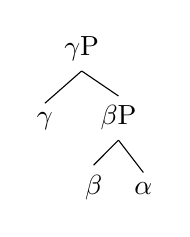
\begin{tikzpicture}[baseline]\tikzset{level distance=25pt, sibling distance=5pt}
\Tree
[.$\gamma$P $\gamma$ [.$\beta$P $\beta$ $\alpha$ ] ]
\end{tikzpicture}
  \caption{Harmonic, right-branching}
  \label{fig:sub1}
\end{subfigure}\hfill
\begin{subfigure}{.25\textwidth}
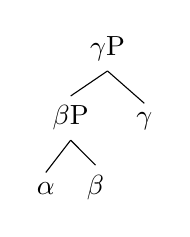
\begin{tikzpicture}[baseline]\tikzset{level distance=25pt, sibling distance=5pt}
\Tree
[.$\gamma$P [.$\beta$P $\alpha$ $\beta$ ] $\gamma$ ]
\end{tikzpicture}
  \caption{Harmonic, left-branching}
  \label{fig:sub2}
\end{subfigure}\hfill
\begin{subfigure}{.25\textwidth}
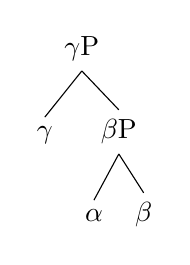
\begin{tikzpicture}[baseline]\tikzset{level distance=30pt, sibling distance=5pt}
\Tree
[.$\gamma$P $\gamma$ [.$\beta$P $\alpha$ $\beta$ ] ]
\end{tikzpicture}
  \caption{Disharmonic, attested}
  \label{fig:sub1}
\end{subfigure}\hfill
\begin{subfigure}{.22\textwidth}
 % \centering
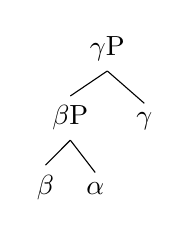
\begin{tikzpicture}[baseline]\tikzset{level distance=25pt, sibling distance=5pt}
\Tree
[.$\gamma$P [.$\beta$P $\beta$ $\alpha$ ] $\gamma$ ]
\end{tikzpicture}
%  \includegraphics[width=.4\linewidth]{image1}
  \caption{Disharmonic, unattested (in relevant domains)}
  \label{fig:sub2}
\end{subfigure}%
\end{figure}

}

In the harmonic (a) and (b) structures in \protect\ref{fofcstructures}, precedence relations are established unproblematically by parameter setting attaching to the c-selection relations between $\beta$ and $\alpha$ and $\alpha$ and $\gamma$, pursuant to \Last[i], in (a), the precedence relations {$\beta$ > $\alpha$ and  $\gamma$ > $\beta$} are established and by transitivity $\gamma$ > $\alpha$. In (b), {$\alpha$ > $\beta$, $\beta$ > $\gamma$} are established by c-selection, and by transitivity $\alpha$ > $\gamma$. In the case of the disharmonic orders in (c) and (d), the condition in \Last[ii] becomes relevant.  In the attested disharmonic order, (c), c-selectional relations will determine the orders $\gamma$ > $\beta$ and $\alpha$ > $\beta$.  C-selectional relations, however, leave underdetermined the relative order of $\gamma$ and $\alpha$, that is, the choice between outputs $\gamma$ > $\alpha$ > $\beta$ and $\alpha$ > $\gamma$ > $\beta$.  The fall back c-command criterion in \Last[ii] however, determines $\gamma$ > $\alpha$. In the disharmonic structure in (d), c-selectional relations will likewise determine $\beta$ > $\gamma$ and $\beta$ > $\alpha$, leaving underdetermined the relative order of $\gamma$ and $\alpha$.  Crucially, the c-command condition in  \Last[ii] will then determine $\gamma$ > $\alpha$, yielding the output $\beta$ > $\gamma$ > $\alpha$ , and \textit{not}, the FOFC-violating order, $\beta$ > $\alpha$ > $\gamma$.  On this approach, the unavailability of FOFC-violating structures in the general case falls out of Sheehan's modified LCA, since the (d) structure in \Last is not linearizable on this approach.\protect\footnotemark\protect\footnotetext{Sheehan does not take up the issue of how to express the exceptionality of A'-movement and c-selectional relations between different extended projections as raised by \cite{biberaueretal2014}.}
	
Sheehan's PF approach and Biberauer et al.'s narrow syntactic approach therefore make different predictions about the reparability of FOFC-violating structures in the syntax.  Again, on the PF approach, but not the narrow syntactic approach a FOFC-violating structure should in principle be derivable in the syntax; it just will not be linearizable.  

One possible case of FOFC repair noted in previous literature involves ``Head-Final Filter'' violations \citep{greenberg1963, williams1982,sheehan2017}.  A well-known restriction on adjectival modification cross-linguistically is a ban on complements of prenominal adjectives where the adjectival complement appears between the adjective and noun. (\cite{williams1982} called this the ``Head-Final Filter''.)  \cite{sheehan2017}, in particular, argues that sentences like \Next[c] should be analyzed as a FOFC effect and proposes an PF approach akin to the one described in section \protect\ref{sheehanpf}.

\exi. 
\a. the proud man
\b. John is proud of his children.
\c. *the [$\gamma$P [$\beta$P proud [$\alpha$P of his children]] man] \\
(adapted from \cite{williams1982})

As Sheehan notes, different languages employ different ``compliance strategies'' for contexts where a Head-final filter would otherwise arise.  One such case involves  extraposition of CP/PP complements of the prenominal adjective as in \Next and \NNext in English and Slovenian respectively.

\ex. \protect\label{extraposition1}
\a. a difficult book [for anyone to read]
\b. *a difficult [for anyone to read] book] \\
(adapted from \cite{sheehan2017})

\exg. \protect\label{extraposition2}\textit{zavesten} \textit{otrok,} \textit{da} \textit{je} \textit{vojna} \\
aware.\textsc{m} child.\textsc{m} that is.\textsc{3sg} war.\textsc{f}\\
`a child aware that there is a war.' \\
(adapted from \citep{sheehan2017})


\cite{sheehan2017} follows \cite{kayne1994} in taking prenominal adjectives to be reduced relative clauses where the adjective raises from a postnominal position. 

\exi. [DP [CP [AP Adj] [NP Noun \st{AP} ]]]


\cite{sheehan2017} proposes that these repair effects might be reconciled with the PF approach to FOFC effects introduced above where FOFC-violating structures are not linearizable by the LCA.  In particular, Sheehan  suggests that the FOFC-violating structures might be repaired at copy deletion by ``scattered deletion'', whereby  ``extraposition'' of the FOFC-offending CP/PP in cases like \protect\ref{extraposition1} and \protect\ref{extraposition2} are achieved by deleting the higher rather than the lower copy of these constituents in order for them to be linearizable by the modified LCA.

In the following discussion, we describe a similar set of facts from Basque verb clusters which suggest that chain reduction may bleed FOFC-violations in a similar way in the absence of scattered deletion.
	

\section{Word order and the functional richness of modal complements in Basque}

The core set of facts that we focus on come from observations by Etxepare, Uribe-Etxebarria and colleagues concerning word order and the functional richness of infinitival complements of the modals  \textit{behar} (`need') and \textit{nahi} (`want') \citep{etxepare-uribeetxebarria2009, etxepare-uribeetxebarria2012, balza2010}.  As illustrated in \Next the constituent headed by \textit{ikusi}, `see', can appear either to the left or the right of the selecting modal, \textit{nahi}, `want'.  

\ex.\protect\label{E-UE-2}\ag. \textit{[Horrelakoak} \textit{maiz-ago}   \textit{ikusi]} \textit{nahi}  \textit{nituzke.} \\
    like.that\textsc{.pl}    often-more see   want  \textsc{aux}     \\ \protect\label{E-UE-2a}
\bg.\textit{Nahi} \textit{nituzke} \textit{[horrelakoak} \textit{maiz-ago} \textit{ikusi.]} \\   
         want  \textsc{aux}      like.that\textsc{.pl}   often-more  see  \\ \protect\label{E-UE-2b}
          `I'd like to see things like that more often.'\\
\citep{etxepare-uribeetxebarria2009}


\cite{etxepare-uribeetxebarria2009, etxepare-uribeetxebarria2012} and \cite{balza2010} note that the word order difference illustrated in \Last correlates with three other properties suggesting that the modal-infinitival order in \Last[b] can involve a functionally richer infinitival complement than \Last[a].  We describe these in  turn below.

\subsection{Temporal modification}

A first way in which infinitival>modal and modal>infinitival orders differ is in terms of the temporal independence of the non-finite constituent.  In infinitival>modal orders, the infinitival phrase cannot contain a temporal modifier forcing a temporal interpretation of the event in the infinitival phrase that is different from that of the modal+auxiliary.  In \Next[a], the infinitival phrase contains \textit{gaur}, `today' with a temporal interpretation different from the past interpretation of the modal+auxiliary, and the result is poor.  On the other hand, Etxepare and Uribe-Etxebarria report that this temporal difference is fine in modal>infinitival contexts such as \Next[b].

\ex.	\ag.\textit{	*Jon-ek} \textit{atzo} \textit{[gaur}    \textit{etxe-a-n}     \textit{ego-n]}        \textit{behar} \textit{zuen.} \\
	Jon-\textsc{erg} yesterday today house-\textsc{def}-in be-\textsc{infin} need   \textsc{aux}    \\
\bg.	\textit{Jon-ek}    \textit{atzo}         \textit{behar}  \textit{zuen}  \textit{[gaur}   \textit{etxe-a-n }        \textit{ego-n.]} \\
	Jon-\textsc{erg} yesterday need   \textsc{aux}   today house-\textsc{def}-in be-\textsc{infin} \\
	`Yesterday Jon needed to be home today.' \\
\citep{etxepare-uribeetxebarria2009}

\cite{etxepare-uribeetxebarria2009, etxepare-uribeetxebarria2012} take these facts to indicate that, in modal>infinitival orders, the non-finite constituent may contain a T head with a tense value different from that of the matrix clause.  In infinitive-modal orders, on the other hand, the non-finite constituent cannot contain a separate T head.



\subsection{Agreement}

A second difference between the word orders concerns agreement.  Open class finite verbs in Basque are formed periphrastically, with a verb root (bearing any aspectual morphology) separate from the auxiliary that agrees in person and number with ergative, absolutive and dative arguments of the main verb.  We illustrate this agreement in \Next.\protect\footnotemark\protect\footnotetext{On a closed class of synthetic verbs, tense and agreement marking appear affixed to the verb root in some aspectual contexts.  Addressee agreement works similarly for these forms but we set these forms aside for expositional convenience.} In the examples in \Next, ergative, absolutive and dative arguments are all overt, however, we note that Basque allows pro-drop with all three of these argument types. 
 
\ex. \label{agreement} \ag. \textit{Ni} \textit{joa-n} \textit{na-iz.}\\	
	     \textsc{1sg.abs} go.\textsc{perf} \textsc{1sg.abs-root}\\
	     `I have gone.'  \hfill{[unaccusative]}
	  \bg. \textit{Katu-ek} \textit{ni} \textit{ikus-i} \textit{na-u-te.}\\	
	      cat-\textsc{3pl.erg} \textsc{1sg.abs} see-\textsc{perf} \textsc{1sg.abs-root}-\textsc{3pl.erg}\\
           `The cats have seen me.' \hfill{[monotransitive]}
         \cg. \textit{Ni-k} \textit{liburu-ak} \textit{Jon-i} \textit{ema-n} \textit{d-i-zki-o-t.}\\	
	      \textsc{1sg-erg} books-\textsc{pl.abs} Jon-\textsc{dat} give-\textsc{perf} \textsc{3sg.abs-root-abs.pl}-\textsc{3sg.dat}-\textsc{1sg.erg} \\
           `I have given Jon the book.'  \hfill{[ditransitive]}
         \dg. \textit{Ni} \textit{Jon-i} \textit{mintza-tzen} \textit{na-tzai-o.}\\	
		\textsc{1sg.abs} Jon-\textsc{dat} speak-\textsc{imperf} \textsc{1sg.abs-root}-\textsc{3sg.dat}   \\
		`I speak to Jon.'   \hfill{[applicative unaccusative]}


In addition, modal verbs that take infinitival complements are transparent to plural absolutive and dative agreement marking in transitive constructions.  In sentences with the modal \textit{behar} `must,'  agreement marking on the auxiliary is exhaustively determined by the argument structure of the lower verb as shown in \Next, below.  

\ex. 	\ag. \% \textit{Joan} \textit{behar}   \textit{na-iz.}	\\						
    go    must   \textsc{1sg.abs-root}\\
    `I must go.'\footnote{In some dialects, the modal \textit{behar} determines the transitive auxiliary \textit{*edun} in unaccusative contexts.}   \hfill{[unaccusative]}
    \bg. \textit{Katu-ek} \textit{ni} \textit{ikusi} \textit{behar} \textit{na-u-te.}\\	
	      cat-\textsc{3pl.erg} \textsc{1sg.abs} see need \textsc{1sg.abs-root}-\textsc{3pl.erg}\\
           `The cats must see me.' \hfill{[monotransitive]}
\cg. \textit{Jon-i}       \textit{liburu-ak}       \textit{eman} \textit{behar}   \textit{d-i-zki-o-t.}			\\
    Jon-\textsc{dat} books-\textsc{pl.abs}  give    need  \textsc{3.abs-root-pl.abs-3sg.dat-1sg.erg}  \\
    `I must give Jon the books.'   \hfill{[ditransitive]}


As \cite{etxepare-uribeetxebarria2009} note, both absolutive plural agreement and dative agreement patterns are constrained by the position of the infinitival.  As shown in \Next, in the modal>infinitival order, absolutive plural agreement is optional.

\ex. 	\ag. 	\textit{Nahi}    \textit{n-\textbf{it}-u-z-ke                                         } \textit{[horr-ela-ko-a-k }           \textit{maiz-ago }         \textit{ikus-i].}        \\
	want   \textsc{1sg.erg-\textbf{pl.abs}-root-pl.abs-irr}    that-like-\textsc{gen-def-pl}  frequent-more see-\textsc{infin} \\
	\bg. 	\textit{Nahi}    \textit{n-u-ke}                      	   \textit{[horr-ela-ko-a-k}                \textit{maiz-ago}          \textit{ikus-i].} \\
  	want   \textsc{1sg.erg-root-irr}    that-like-\textsc{gen-def-pl}  frequent-more see-\textsc{infin} \\
		`I'd like to see things like that more often.'\\
\citep{etxepare-uribeetxebarria2009}

In the infinitival>modal order, on the other hand, plural absolutive agreement on the auxiliary is obligatory.

\ex.	\ag. 	\textit{[Horr-ela-ko-a-k }             \textit{maiz-ago}         \textit{ikus-i]}         \textit{nahi}    \textit{n-\textbf{it}-u-z-ke.}  \\
     that-like-\textsc{gen-def-pl}  frequent-more see-\textsc{infin}  want     
        \textsc{1sg.erg-\textbf{pl.abs}-root-pl.abs-irr}    \\
     	\bg. \textit{*[Horr-ela-ko-a-k}              \textit{maiz-ago}         \textit{ikus-i]}         \textit{nahi}   \textit{nuke.}   \\  
       that-like-\textsc{gen-def-pl}  frequent-more see-\textsc{infin}  want \textsc{1sg.erg-root-irr}  \\   
      `I'd like to see things like that more often.' \\
	\citep{etxepare-uribeetxebarria2009}


Agreement with dative arguments is similarly constrained.  \Next shows that that dative agreement is optional in the modal>infinitival order. 

\ex. 	\ag. 	\textit{Behar}  \textit{zen-i-e-ke} 		             \textit{[zure guraso-ei}              \textit{obeditu].} \\
             	must   \textsc{2abs-root-dat.pl-irr}    your parent-\textsc{dat.pl}   obey  \\
	\bg.	\textit{Behar} \textit{zen-u-ke} 	         \textit{[zure} \textit{guraso-ei} \textit{obeditu].} \\
	    must   \textsc{2abs-root-irr}   your parent-\textsc{dat.pl}   obey    \\    
	 	`You should obey your parents.'\\
			\citep{etxepare-uribeetxebarria2009}

	As shown in \Next, this agreement is obligatory when the order is infinitival>modal:

\ex. 	\ag. \textit{[Zure} \textit{guraso-ei}              \textit{obeditu]} \textit{behar}  \textit{zen-i-e-ke.}  \\
             	your parent-\textsc{dat.pl}   obey     must   \textsc{2sg.abs-root-dat.pl-irr}  \\
	\bg.	\textit{[*Zure} \textit{guraso-ei} \textit{obeditu]} \textit{behar} \textit{zen-u-ke.} \\
	    your parent-\textsc{dat.pl}   obey     must   \textsc{2sg.abs-root-irr}  \\
		`You should obey your parents.'  \\
			\citep{etxepare-uribeetxebarria2009}


These agreement restrictions stand to reason on the assumption that the loci for dative and absolutive case in transitive contexts is not T but rather some set of vP-internal heads---v and Appl for instance---and that the agreement morphemes on the auxiliary reflect head movement from v/Appl to T \citep{arregi-molinaazaola2004, rezac2008}.  On this approach, the unavailability of dative and plural absolutive agreement on the finite auxiliary plausibly reflects the presence of a lower T blocking movement to the higher T.

\subsection{Negation}

	 The above sets of facts plausibly indicate that in modal>infinitival but not infinitival>modal orders, the non-finite constituent may contain a T head.  A final set of facts, however, suggests that in modal-infinitive orders, the non-finite constituent can be somewhat larger than TP--containing minimally a TP-external negation projection. \cite{balza2010} and \cite{etxepare-uribeetxebarria2009} observe that non-finite constituents to the left of the modal can never contain the sentential negation morpheme \textit{ez}, which appears to the left of the auxiliary in Basque \citep{laka1990}.  In contrast, when the infinitive appears to the right of the modal, \textit{ez} can indeed appear.  This contrast is illustrated in \Next.  

\ex.	\ag.	\textit{*[Ez} \textit{eros-i]}           \textit{nahi/behar} \textit{n-u-ke.}\\
   	\textsc{neg} buy-\textsc{infin} want/need   \textsc{1sg.erg-root-irr}   \\
\bg.	\textit{Nahi/behar} \textit{n-u-ke} \textit{[ez} \textit{eros-i].}\\
     want/need  \textsc{1sg.erg-root-irr}    \textsc{neg} buy-\textsc{infin} \\
     `I want/need not to buy it.' \\\citep{etxepare-uribeetxebarria2009}

As \cite{etxepare-uribeetxebarria2009} note, the negation in \Last[b] is not plausibly an instance of constituent negation since constituent negation does not license a higher, clausemate negative polarity item (NPI).  Example \Next[a], illustrating constituent negation in a non-modal context, shows that the higher NPI \textit{inork}, `anyone' is not licensed, unlike a true sentential negation context such as \Next[b].  

\ex.	\ag.	\textit{*Inork} \textit{(ere)}     \textit{du}     \textit{ez}  \textit{eros-i.} \\
   	Nobody (at-all) \textsc{aux} \textsc{neg} buy-\textsc{infin} \\
       `Nobody at all bought it.' 
	\bg. 	\textit{Inork} \textit{(ere)}       \textit{ez}    \textit{du}   \textit{eros-i.}   \\
		Nobody (at-all) \textsc{neg} \textsc{aux} buy-\textsc{infin}  \\
   	`Nobody at all bought it.'


\Next shows that \textit{ez} in modal>infinitival contexts behaves like sentential negation in licensing the higher NPI, \textit{deus}, `anything'.  \cite{balza2010} and \cite{etxepare-uribeetxebarria2009} take these facts to indicate that the non-finite constituents in these environments can contain a negative head.

\exg.	\textit{Nahi}  \textit{nuke} \textit{deus} \textit{(ere)} \textit{ez} \textit{eros-i.}\\
want \textsc{aux}   nothing at.all \textsc{neg} buy-\textsc{infin} \\
	`I'd like to not buy anything (at all).'


To summarize, we have described four sets of facts drawn mainly from  \cite{etxepare-uribeetxebarria2009, etxepare-uribeetxebarria2012} and \cite{balza2010} suggesting that the two word orders discussed above correspond to different internal structures of the non-finite constituent. The infinitival phrase in infinitival>modal orders is smaller than TP---a vP, we'll assume---while the infinitival in modal>aux>infinitival orders can be a TP and may contain a TP-external negation position as well.  We illustrate this proposal with the sequences of functional heads in \protect\ref{structuresensitivity}, (repeated here) which abstract away from surface linear order.

\ex.	\protect\label{structuresensitivity} \a. \textbf{Infinitival>modal orders:} [T [Modal [v [V \ldots  
	\b. \textbf{Modal>infinitival orders:} [T [Modal ([Neg) ([T)  [v [V \ldots  \\


As noted earlier, \cite{balza2010} and \cite{etxepare-uribeetxebarria2009} do not provide an account of the contrast in \Last.  In the following discussion, we argue that this contrast is explainable as a garden variety FOFC effect from the perspective of antisymmetric approaches to Basque.

\section{FOFC and word order in Basque verb clusters}
\subsection{Antisymmetry and polarity-sensitive word order alternations}

Basque is a ``mixed-head'' language: heads in the clausal spine below T appear to the right of their complements, while heads above T, including preverbal speech act and evidential particles appear to the left of their complements \citep{derijk1969, ortizdeurbina1989, ortizdeurbina1994, laka1990,elordieta2001, irurtzun2007, elordieta2008} . Most generative approaches to Basque have modeled these facts in terms of a head-directionality parameter: T and clausal heads below it take their complements to the left, while those heads above T take their complements to the right. The head-final nature of TP-internal projections, on this approach, usefully accounts the fact that in neutral declarative sentences like \protect\ref{affirmativeclauses}, the finite verb--presumably in T--appears sentence finally.

\ex. \textbf{\textit{Affirmative main clauses}} \protect\label{affirmativeclauses}\samepage

\exg.[{}] \textit{Miren-ek}   \textit{Jon} \textit{ikus-i}      \textit{du.}   \\				
         Miren-\textsc{erg} Jon-\textsc{abs} see-\textsc{perf}   \textsc{aux}.\textsc{3sg.erg} \\
         `Miren has seen Jon.'


In negative sentences, the negative morpheme \textit{ez} appears left-adjacent to the auxiliary and the VP appears to the right of the auxiliary as in \Next.

\ex. \textbf{\textit{Negative main clauses}}\protect\label{negativeclauses}\samepage

\exg.[{}]   \textit{Miren-ek}   \textit{ez}     \textit{du}   \textit{Jon} \textit{ikus-i.} 	\\			
         Miren-\textsc{erg} \textsc{neg} \textsc{aux}.\textsc{3sg.erg} Jon-\textsc{abs} see-\textsc{perf} \\
         `Miren hasn't seen Jon.'


\cite{laka1990} and \cite{elordieta2001, elordieta2008} propose that these polarity effects reflect the fact that negation---which is head-initial on this approach---is first-merged outside TP in Basque, and that the inflected verb must head adjoin to negation as a way of providing lexical support for the clitic-like auxiliary. The Neg>Aux word order requires that this be right head adjunction as shown in \Next.  In affirmative sentences, Neg is not merged, and the auxiliary stays in its first-merged position in TP.  

\ex. \textbf{\textit{The head movement approach (Laka, 1990)}} \label{tree-2} \\  \samepage
 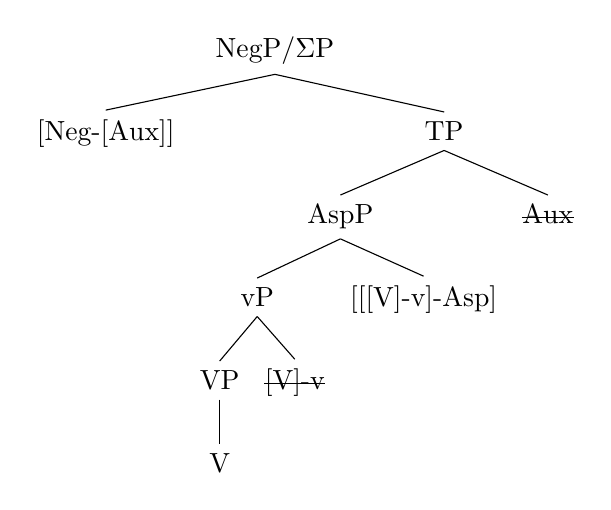
\begin{tikzpicture}[baseline]\tikzset{level distance=30pt, sibling distance=2.5pt}
\Tree
[.{NegP/$\Sigma$P} {[Neg-[Aux]]}  [.TP [.AspP [.vP [.VP V ] {\st{[V]-v}}  ] {[[[V]-v]-Asp]}  ] \st{Aux} ] ]
\end{tikzpicture}
\vspace{.5cm}


%\ex. \textbf{\textit{Negative orders on the head directionality parameter approach}} \label{tree-2} \\  \samepage
%\begin{tikzpicture}[baseline]\tikzset{level distance=25pt, sibling distance=5pt}
%\Tree
%[.NegP [.Neg Neg Aux ] [.TP [.AspP [.vP [.VP \st{V} ] \st{v-V} ] %[.Asp V-v-Asp ] ] \st{Aux} ] ]
%\end{tikzpicture}


On an approach that eschews head-directionality parametrization, a different account is required for the polarity-sensitive word order alternations illustrated in \ref{affirmativeclauses} and \protect\ref{negativeclauses}.  In particular, following \cite{haddican2004a, haddican2008}, we propose that  (i) the left-branching structure of the extended VP is derived via roll up \citep{kayne1994}, and (ii) the relative order of the auxiliary and extended verbal projection reflects the presence or absence of fronting of the extended verbal projection, a constituent that we will label PolP, for reasons to be made clear shortly.  We adopt Laka's seminal proposal that Basque has a left peripheral polarity head, $\Sigma$.  We propose that this head probes for polarity-specified elements.  Two such elements will be the the negative and the emphatic affirmative morphemes \textit{ez} and \textit{bai}, which we take to be  polarity adverbs merged in the Spec of  PolP. These forms, where present will raise to Spec, SigmaP, as illustrated in the negative example in \Next.
	
\ex. \textbf{Ez-\textit{raising, negative contexts}} \protect\label{tree-5} \\  \samepage
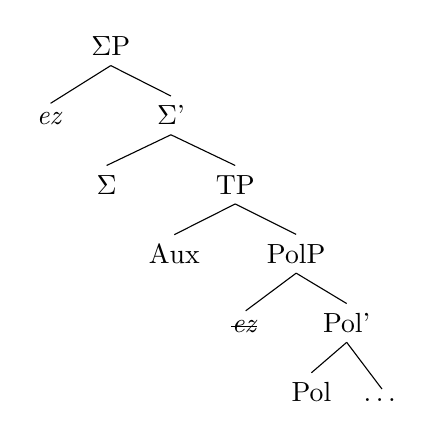
\begin{tikzpicture}[baseline]\tikzset{level distance=25pt, sibling distance=5pt}
\Tree
[.$\Sigma$P \textit{ez} [.$\Sigma$' $\Sigma$ [.TP Aux [.PolP \st{\textit{ez}} [.Pol' Pol {\ldots} ] ] ] ] ]
\end{tikzpicture}

%\vspace{2 cm}


	In affirmative root contexts, the position to the left of the auxiliary is not occupied by the negative morpheme \textit{ez}, but rather by the extended projection of the verb.  We propose that, in these contexts, in the absence of \textit{ez}, the extended verbal phrase raises to \begin{math}\Sigma \end{math} to satisfy the latter's polarity feature.  Specifically, in the spirit of predicate fronting approaches to VSO and VOS word orders  \citep{massam2000, massam2001, massam2010, coon2010, coon2012}, let us assume that what raises is a PolP whose head contains an affirmative polarity [Aff] feature.  In the verb-initial orders they analyze, Massam and Coon take the landing site of this movement to be TP/IP, and relate this movement to the featural needs of T/C.  In Basque, we take this movement to be related to featural needs of a polarity-related morpheme, namely  \begin{math}\Sigma \end{math}. We illustrate this in \Next.\protect\footnotemark \protect\footnotetext{See \cite{haddican2004a, haddican2008} and \cite{etxepare-uribeetxebarria2009} for similar approaches.}
	

\ex. \textbf{\textit{Affirmative orders}} \protect\label{tree-6} \\ \samepage
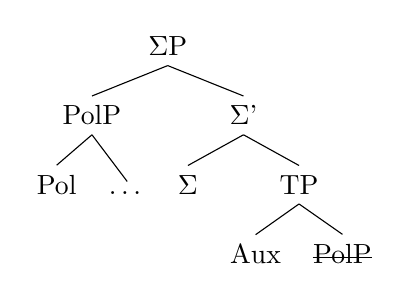
\begin{tikzpicture}[baseline]\tikzset{level distance=25pt, sibling distance=5pt}
\Tree
[.$\Sigma$P [.PolP Pol {\ldots}  ] [.$\Sigma$' $\Sigma$ [.TP Aux \st{PolP} ] ] ]
\end{tikzpicture}


%\vspace{2 cm}


Evidence in favor of predicate fronting in affirmative clauses comes from TP ellipsis sentences like \Next and \NNext. In both cases, the auxiliary in the second sentence is left unpronounced, plausibly as a banal case of TP ellipsis \citep{laka1990}.  Interestingly, the elements which escape TP-ellipsis are different in affirmative and negative sentences: whereas in negative sentences (and in those involving contrastive affirmation) the verbal predicate is elided together with the finite auxiliary \NNext, in simple affirmative sentences the verbal predicate escapes TP-ellipsis, by virtue of obligatory predicate raising \Next. On the head directionality approach, additional movement operations are required to derive such sentences.

\exig. \textit{Jon-ek} \textit{kafe-a} \textit{erosi} \textit{du,} \textit{eta} \textit{Ane-k,} \textit{[$\Sigma$P} \textit{[PolP} \textit{[} \textit{liburu-a} \textit{leitu]} \textit{$\Sigma$} \textit{\st{[$\mathrm{_T}$$\mathrm{_P}$} \textit{du} }\textit{].} \\
	Jon-\textsc{erg} coffee bought \textsc{aux} and Ane-\textsc{erg} \textcolor{white}{x} \textcolor{white}{x} {}
book-the read\\
\vspace*{-.45cm}`Jon has bought coffee, and Ane has read the book.'

\exig. J\textit{on-ek} \textit{kafe-a} \textit{erosi} \textit{du,} \textit{baina} \textit{Ane-k,} \textit{[$\Sigma$P}  \textit{ez} \textit{$\Sigma$} \textit{\st{[$\mathrm{_T}$$\mathrm{_P}$ du kafe-a erosi]}.} \\
	Jon-\textsc{erg} coffee bought \textsc{aux} but Ane-\textsc{erg}  \textcolor{white}{x} \textcolor{white}{x} \textsc{neg} \\ %\textcolor{white}{$\Sigma$} \textcolor{white}{x} \textsc{aux} coffee-the bought\\
	\vspace*{-.45cm}`Jon has bought coffee, but Ane hasn't.'

Evidence that the extended VP indeed contains a polarity feature in affirmative contexts comes from polarity focus sentences like \Next.  Here, the extended VP raises to a left peripheral focus position and co-occurs with an affirmative denial interpretation, suggesting the raised verbal constituent is the locus of the affirmative feature.

\exig. \textit{[FocP} \textit{[PolP} \textit{Etorri]} \textit{[TP} \textit{da} \textit{Iker]].} \\
	{} {} come {} \textsc{aux} Iker\\
	`Iker HAS (indeed) come.' \protect\label{iker}


What is important about this approach for the FOFC-effects focused on here is that TP is a left-headed projection that does not participate in roll-up movement; that is, the complement of T does not move to its spec.  From this perspective, and assuming that non-fintite T is like finite T in not participating in roll-up movement, Etxepare and Uribe-Etxebarria's observed correlation between word order and size of the modal complement is explicable as a vanilla FOFC effect.  That is, what makes the functionally richer constituents impossible in the infinitive>modal order is the presence of a head-complement structure in the spec of the modal phrase, in violation of \protect\ref{fofc2}.  Specifically, the complement of the infinitival T is not spelled out in the spec of the non-finite T, but rather as the sister of T.  The infinitival T itself then moves to the spec of the modal projection and runs afoul of \protect\ref{fofc1}. In contrast, vP-sized infinitives will not run afoul of FOFC, as stated in \protect\ref{fofc1} and \protect\ref{fofc2}, since v \textit{does} participate in roll-up; that is, it attracts its complement to its spec. We illustrate this proposal in \Next and \NNext.


\ex. \textbf{\textit{FOFC-violating TP-raising}} \protect\label{tree-8} \\  \samepage
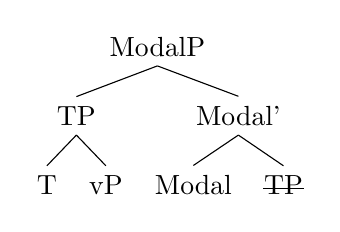
\begin{tikzpicture}[baseline]\tikzset{level distance=25pt, sibling distance=5pt}
\Tree
[.ModalP [.TP T vP ] [.Modal' Modal \st{TP} ] ]
\end{tikzpicture}

\vspace{.5cm}
 
\ex. \textbf{\textit{FOFC-compliant vP-raising}} \protect\label{tree-9} \\  \samepage
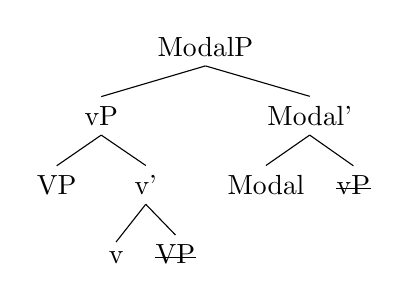
\begin{tikzpicture}[baseline]\tikzset{level distance=25pt, sibling distance=5pt}
\Tree
[.ModalP [.vP VP [.v' v \st{VP} ] ] [.Modal' Modal \st{vP} ]  ]\end{tikzpicture}

\vspace{.5cm}


From the perspective of the antisymmetric approach to polarity-sensitive word order alternations described above, the structure-sensitivity of the word order alternations described by \cite{etxepare-uribeetxebarria2009} is therefore predicted as a FOFC effect. From a mixed head perspective, where T takes its complement on the left, some other account of Etxepare and Uribe-Etxebarria's observation is required.\protect\footnotemark\protect\footnotetext{For the same reason, Sheehan's (2013a, b) approach will fail to express the structure-sensitivity of these word order alternations as a FOFC phenomenon if T is parameterized to take its complement to its left.  Sheehan's theory, though, entails no commitment to such a derivation versus an XP movement approach of the kind just proposed.}


\subsection{Repairing the violation}

The account so far explains why vP--, but not TP-sized modal complements can raise to the specifier of the modal.  Unaddressed so far is why TP-sized modal complements are licit when they appear to the right of the modal as in \protect\ref{E-UE-2b}.  A further fact about the alternation in \protect\ref{E-UE-2} that we take to be central to this issue is the fact that the modal-aux-infinitive order is most readily available in contexts in which the non-finite constituent to the right is focalized or contains a focus-bearing constituent. The modal+auxiliary sequence to the left is preferably defocused.  From this perspective, sentences like \protect\ref{E-UE-2b} are reminiscent of cases of right peripheral focus constructions as in \Next and \NNext.


\exg. \textit{Ardoa} \textit{ekarri} \textit{diot} \textit{(\#)} \textit{ANDONI-RI.} \\
wine brought \textsc{aux} {} Andoni-\textsc{dat} \\
I brought the wine to ANDONI. \\
\citep{elordieta2001}

\exg. \textit{Monjak} \textit{egin} \textit{zigun} \textit{[barruan} \textit{utz-i.]} \\
nuns do \textsc{aux} inside leave-\textsc{infin} \\
The nuns LEFT US INSIDE. \\
\citep{haddican2007}


\cite{ortizdeurbina2002}, \cite{uribeetxebarria2003} propose that sentences such as \LLast and \Last are derived by movement of the focused constituents to a left-peripheral focus position, followed by remnant movement of the non-focused portion of the sentence to a higher topic phrase.  We illustrate this proposal in \Next. As \cite{ortizdeurbina2002} notes, this approach is supported by the fact that the remnant-moved material shares intonational properties with other pre-focus topic constituents.  

\exig. [TopP [ \textit{Ardoa} \textit{\st{Andoni-ri}} \textit{ekarri} \textit{diot]} \textit{Top} [FocP \textit{[} \textit{Andoni-ri} \textit{]}\ldots  \textit{]}  \\
{} {} wine {} brought \textsc{aux} {} {} {} Andoni-\textsc{dat} \\\protect\label{ardoa}
I brought the wine to ANDONI. 
	
	
	Some support for remnant movement comes from the relative scope of focus and negation. When following the lexical verb, the favored scope of the focal constituent is maximal with regard to negation, as diagnosed by the continuation \textit{and not DP}. In this regard, it behaves like left-peripheral foci as in \Next[b] \citep{ortizdeurbina2002}.
	
\ex.	
\ag. \textit{Ez} \textit{diot} \textit{liburua} \textit{oparitu} \textit{ANDONI-RI,} \textit{eta} \textit{ez} \textit{Miren-i.}\\
\textsc{neg} \textsc{aux} book-the offered Andoni-\textsc{dat}, and \textsc{neg} Miren-\textsc{dat}\\
`The one I did not offer the book to is Andoni, and not Miren'
\bg. \textit{ANDONI-RI} \textit{ez} \textit{diot} \textit{liburua} \textit{oparitu,} \textit{eta} \textit{ez} \textit{Miren-i.}\\
Andoni-\textsc{dat} \textsc{neg} \textsc{aux} book-the offered and \textsc{neg} Miren-dat\\
`It is Andoni that I didn't offer the book to, and not Miren'
	
	
Also, note that wide-scope foci in non-initial position must occupy the right edge of the clause as suggested by the fact that they cannot be followed linearly by clausal material:


\ex.
\ag. \textit{Jon-ek} \textit{ez} \textit{du} \textit{liburu-rik} \textit{irakurri} \textit{BULEGOAN,} \textit{eta} \textit{ez} \textit{trenean.}\\
Jon-\textsc{erg} \textsc{neg} \textsc{aux} book-\textsc{infin} read office-in and \textsc{neg} train-in\\
`The place Jon did not read any book is the office, not the train'
\bg. \textit{Jon-ek} \textit{ez} \textit{du} \textit{irakurri} \textit{(liburu-rik)} \textit{BULEGOAN} \textit{(*liburu-rik),} \textit{eta} \textit{ez} \textit{trenean.}\\
Jon-\textsc{erg} \textsc{neg} has read book-part office-in book-\textsc{part} and \textsc{neg} train-in\\
`The place Jon did not read any book is the office, not the train'	
	
	
	The crux of our proposal about FOFC repair is as follows.  In modal>infinitival orders such as \protect\ref{E-UE-2b}, affirmative PolP moves to \begin{math}\Sigma \end{math}P, as usual. The FOFC-offending infinitival TP then subextracts to a Focus phrase, as in \Next. The position of the modal to the left of the infinitival is derived via remnant topicalization, not shown here. Crucially, because the TP targets an A-bar position, this movement step is FOFC-exempt. (See \cite{biberaueretal2014} for discussion.)

\ex. \textbf{\textit{PolP movement to \begin{math} \bf{\it{\Sigma}}\end{math}P and sub-extraction of infinitival TP}} \\
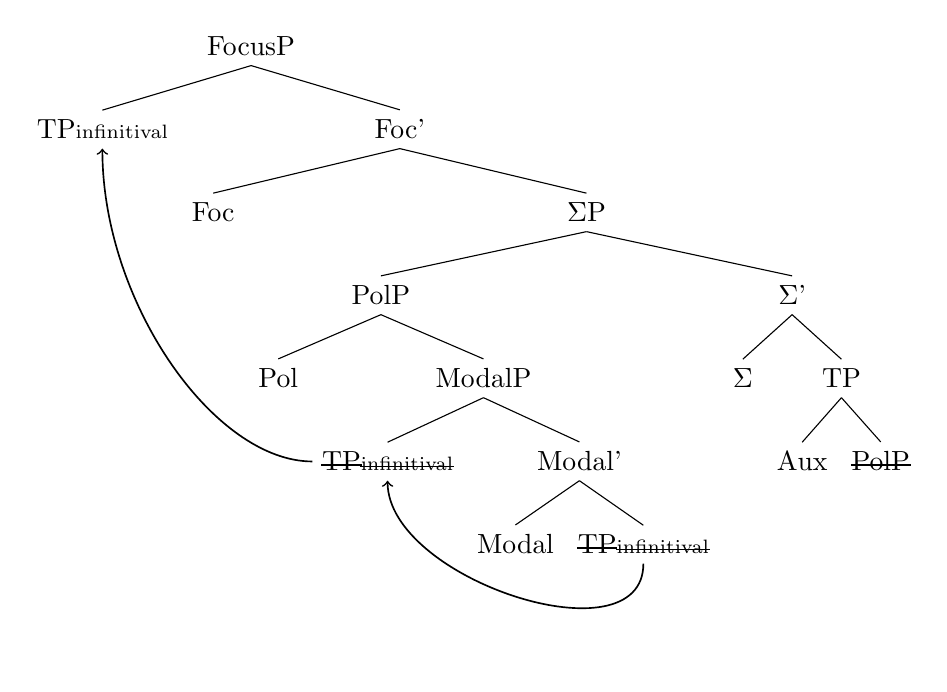
\begin{tikzpicture}
\Tree
[.FocusP \node(infin-3){TP\scriptsize{infinitival}}; [.Foc' Foc [.$\Sigma$P [.PolP Pol [.ModalP \node(infin-2){\st{TP}\scriptsize{\st{infinitival}}}; [.Modal' Modal \node(infin-1){\st{TP}\scriptsize{\st{infinitival}}}; ] ] ]  [.$\Sigma$' $\Sigma$ [.TP Aux \st{PolP} ] ] ] ] ]
\draw[semithick,->] (infin-1)..controls +(south:1.5) and +(south:1.5)..(infin-2);
\draw[semithick,->] (infin-2)..controls +(west:2.2) and +(south:2.2)..(infin-3);
\end{tikzpicture}



The derivation in \Last requires that freezing effects do not apply in this context \citep{collins2005b, collins2005a}.  We do not consider in detail what conditions the availability of subextraction here, but note that independent evidence of the ability of focused constituents to extract from moved XPs come from examples like \Next and discussed by \cite{elordieta2008}.  Here, the \textit{wh-}phrase, \textit{norekin}, `with who' cyclically moves from within a moved CP.

\exig.  \textit{Nor-ekin} \textit{pentsa-tu} \textit{duzu} \textit{[CP} \textit{\st{nor-ekin}} \textit{ezkondu} \textit{behar} \textit{naiz-ela]} \textit{agindu} \textit{didate-la} \textit{\st{CP}?}\\
          who-with think-\textsc{perf} \textsc{aux} \textcolor{white}{text}  who-with marry must \textsc{aux-C} order \textsc{aux-C}\\
`Who did you think they told me I had to get married with.'


Subextraction of TP to the Focus Phrase is followed by remnant topicalization of $\Sigma$P, as in \protect\ref{ardoa}. Evidence that the modal in the relevant cases sits in a derived position comes from complex functional sequences preceding the non-finite constituent that cannot be generated in-situ (Etxepare and Uribe-Etxebarria, 2009). Consider \Next:

	
\exg. \textit{Nahi} \textit{izan}   \textit{du}   \textit{beranduago} \textit{etorri.}	\\
        Want \textsc{perf} \textsc{aux} later            come\\
        		`She/he has wanted to come later.' 


In \Last, the perfect head follows the modal, which it selects, and precedes the auxiliary, which in turn precedes the non-finite verb. The hierarchical relations among the different components of the matrix-clause functional sequence can be represented in terms of either a head-final structure or roll-up movement, but the relative ordering of that sequence and the non-finite verb cannot: the modal verb selects the non-finite TP, but the two elements appear on opposite sides of the sequence, and separated by other clausal heads. Remnant movement provides a simple rationale for this ordering, and is well attested in other Basque focal constructions. \Next lays out the derivational steps necessary to arrive to a configuration such as \Last, starting from the merger of the Modal head with the TP-infinitival \Next[a]:


\exi.
\a. Merge modal \textit{nahi} with infinitival TP:\\
[ModalP \textit{nahi} [TP \textit{etorri} ]]  
\b. Infinitival TP rolls up with ModalP:\\
 [ModalP [TP \textit{etorri}] \textit{nahi} \st{TP}
\c. Merge Aspect (participle \textit{izan}):\\
 [AspP \textit{izan} [ModalP [TP \textit{etorri} ] \textit{nahi}  ]] 
 \d. ModalP rolls up with AspP:\\
 [AspP [ModalP [TP \textit{etorri} ] \textit{nahi} ]  \textit{izan} \st{ModalP}  ]
 \e. Merge Pol and finite auxiliary in T:\\
 [TP \textit{du} [PolP Pol [AspP [ModalP [TP \textit{etorri} ] \textit{nahi} ]  \textit{izan}   ]]]
\f. Merge $\Sigma$:\\
 [$\Sigma$P $\Sigma$ [TP \textit{du} [PolP Pol [AspP [ModalP [TP \textit{etorri} ] \textit{nahi} ]  \textit{izan} ]]]]
\f. Predicate fronting---PolP raising to $\Sigma$P:\\
 [$\Sigma$P  [PolP Pol [AspP [ModalP [TP \textit{etorri} ] \textit{nahi} ]  \textit{izan}   ]] $\Sigma$ [TP \textit{du} \st{PolP} ]]
\f. Merge focus head and move infinitival TP to spec, Foc:\\
 [FocP [TP \textit{etorri}] Foc [$\Sigma$P [PolP Pol [AspP [ModalP \st{\textit{etorri}} \textit{nahi} ]  \textit{izan}]] $\Sigma$ [TP \textit{du} ]]]
 \f. Merge Topic head and remnant move $\Sigma$P to spec, Topic:\\
 [TopP   [$\Sigma$P [PolP Pol [AspP [ModalP  \textit{nahi} ]  \textit{izan}]] $\Sigma$ [TP \textit{du} ]] Top [FocP [TP \textit{etorri}] Foc \st{$\Sigma$P}]

 
To summarize, the importance of the foregoing facts for the debate between narrow syntactic and PF-based approaches to FOFC is that they suggest a derivation whereby a FOFC-violating structure is assembled, but then repaired by a subsequent movement step. The analysis, if correct, entails that Biberauer et al.'s narrow-syntax approach to FOFC, where FOFC-violating structures are simply not buildable in the syntax, cannot be correct. Rather, they suggest that copy-deletion can bleed FOFC. This, in turn, means that FOFC-evaluation is derivationally subsequent to copy-deletion, in the phonological component of the grammar on standard approaches \citep{nunes2004}.
	
	


\section{Conclusion}
This paper has presented an analysis of word-order restrictions in Basque modal constructions described in recent work by \cite{etxepare-uribeetxebarria2009, etxepare-uribeetxebarria2012}.  We have shown that the relevant restrictions are explained as an utterly banal FOFC effect on antisymmetric approaches to Basque, but not on a traditional mixed head approach.  The analysis of Basque verb clusters presented, if correct, entails that Biberauer et al.'s narrow syntactic approach to FOFC effects is not correct and instead recommends a PF-based approach. How this might be achieved, whether by Sheehan's promising analysis (\citeyear{sheehan2013a,sheehan2013b}) or another approach might usefully be investigated in future work.
	
\section*{Acknowledgements}
	
	
	Many  thanks Be\~nat Oyhar\c cabal members of the Basque Dialect Grammar team and an audience at GLOW. This research is supported by a grant from the Spanish Ministerio de Ciencia e Innovaci\'on FFI2008-00240/FILO, FFI2008-05135/FILO and from the Basque Government GIC07/144-IT-210-07. All errors are our own.
	
\printbibliography[heading=subbibliography,notkeyword=this]

%\bibliography{anders}
%\bibliography{/Users/williamhaddican/Dropbox/syntax}
%\bibliographystyle{biblatex-langsci-unified}



\end{document}  